\Chapter{Szoftverhasználat}

\begin{multicols}{2}
[
 A szoftver kezelőfelülete kifejezetten intuitívra lett tervezve, egyszerűen lehet vezé\hyp{}relni a programot, illetve megtalálni benne az egyes funkciókat.Az alábbi ábrán látható az a felület ami a program elindításakor nyílik meg.
]
	
	\begin{Figure}
		\centering
		\captionof{figure}{Kezdeti felület}
		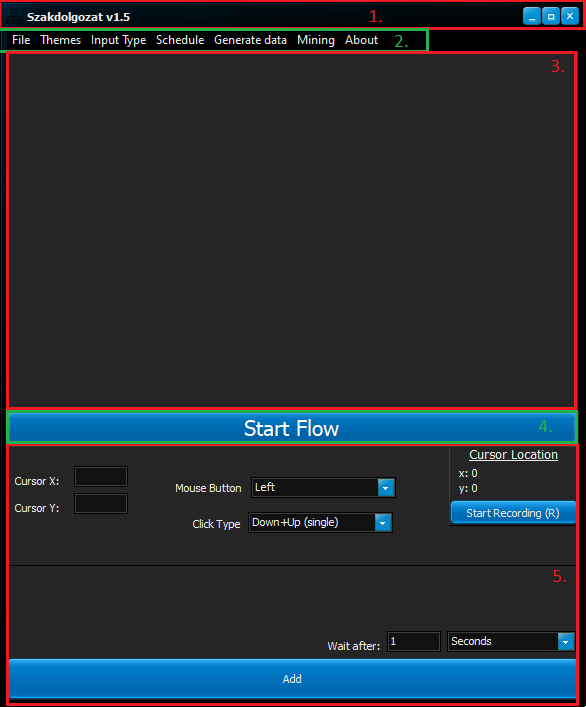
\includegraphics[width=\linewidth, keepaspectratio=true]{images/img_ui_1}	
		\label{fig:ui}
	\end{Figure}
	
	\textbf{Magyarázat}
	\begin{enumerate}
		\item{Fejléc \& rendszer menü}
		\item{Főmenü}
		\item{Folyamati panel}
		\item{Folyamat indító gomb}
		\item{Lépés hozzáadása - egér}
	\end{enumerate}

\end{multicols}

\Section{Főmenü}

Miután a program elindult, a különböző funkciók közötti navigálásra a főmenüt lehet használni. Ennek a használata az alábbiak alapján működik:
\begin{enumerate}
	\item{
		\textbf{File}: Itt van lehetőség a folyamatok külön fájlokként való kezelésére.
		\begin{figure}[h]
			\begin{center}
				\caption{"File" menü}
				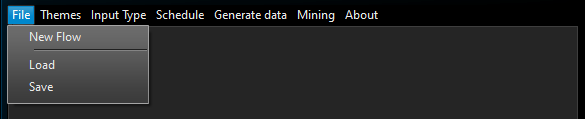
\includegraphics[width=0.5\textwidth, keepaspectratio=true]{images/img_ui_file}\\
				\label{fig:example}
			\end{center}
		\end{figure}

		Lehet: 
		\begin{itemize}
			\item{Új folyamatot létrehozni,}
			\item{Folyamatot fájlból betölteni,}
			\item{Folyamatot lementeni állományba.}
		\end{itemize}
	}
	\item{
		\textbf{Themes}: Ebben a menüben a szoftver felületének a megjelenítését lehet változ\hyp{}tatni. Számos beépített témával rendelkezik amiből választani lehet a felhasználó kedvére.
		\begin{figure}[h]
			\begin{center}
				\caption{"Themes" menü}
				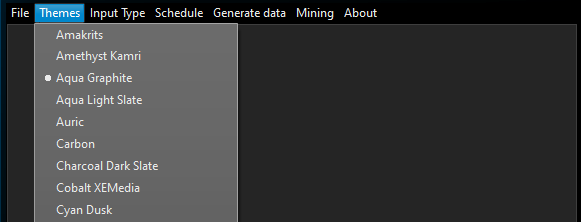
\includegraphics[width=0.5\textwidth, keepaspectratio=true]{images/img_ui_themes}\\
				\label{fig:example}
			\end{center}
		\end{figure}
	}
	\item{
		\textbf{Input Type}: Van lehetőség a jelenlegi folyamathoz kézileg hozzáadni lépést, vagy hozzáfűzni olyan lépéseket amiket a program generál miután rögzítette a felhasználó eseménysorát. Ezeket a funkciókat érjuk el ezzel a menüvel.
		\begin{figure}[h]
			\begin{center}
				\caption{"Input type" menü}
				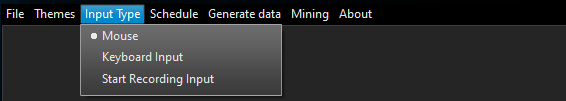
\includegraphics[width=0.5\textwidth, keepaspectratio=true]{images/img_ui_input}\\
				\label{fig:example}
			\end{center}
		\end{figure}
		\begin{itemize}
			\item{\textbf{Mouse}: Egérkattintások hozzáadása kézileg}
			\item{\textbf{Keyboard Input}: Billentyű lenyomások hozzáadása kézileg}
			\item{\textbf{Start Recording Input}: Felhasználói eseménysor rögzítése, majd befejezés után lépések generálása.}
		\end{itemize}
	}
	\item{
		\textbf{Schedule}: Itt érhető el a folyamatok időzítésére szolgáló felület.
		\begin{figure}[h!]
			\begin{center}
				\caption{"Schedule" menü}
				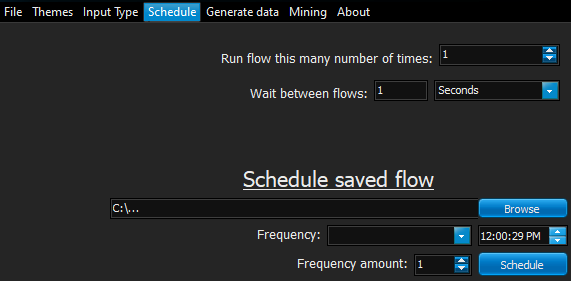
\includegraphics[width=0.3\textwidth, keepaspectratio=true]{images/img_ui_schedule}\\
				\label{fig:example}
			\end{center}
		\end{figure}
	}
	\item{
		\textbf{Generate data}: Folymatokat lehet itt generálni előre meghatározott forgató\hyp{}könyvek alapján.
		\begin{figure}[h!]
			\begin{center}
				\caption{"Generate Data" menü}
				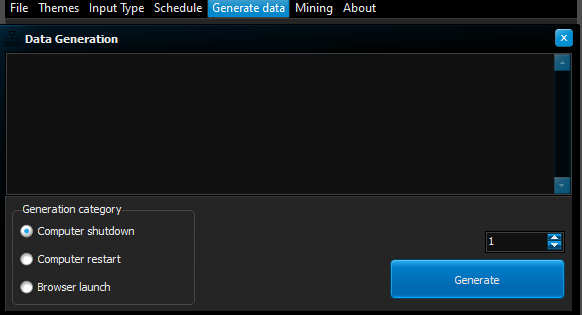
\includegraphics[width=0.5\textwidth, keepaspectratio=true]{images/img_ui_datagen}\\
				\label{fig:example}
			\end{center}
		\end{figure}
	}
	\item{
		\textbf{Mining}: Az adatbányászatra szólgáló felületet itt érjük el.
		\begin{figure}[h!]
			\begin{center}
				\caption{"Mining" menü}
				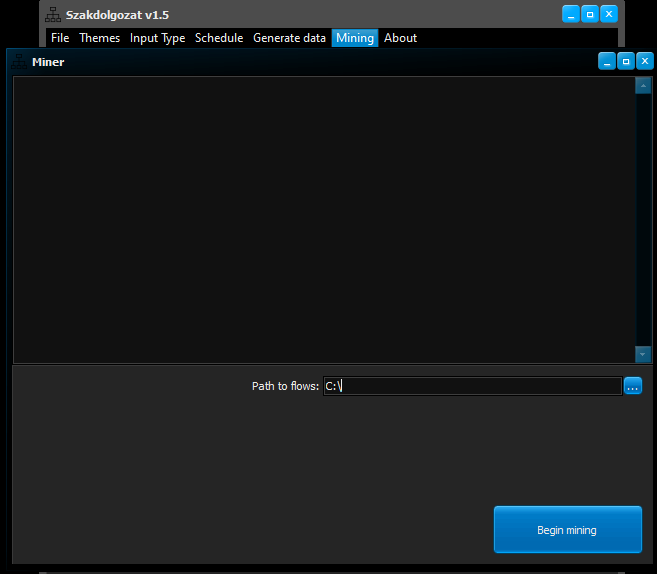
\includegraphics[width=0.5\textwidth, keepaspectratio=true]{images/img_ui_mining}\\
				\label{fig:example}
			\end{center}
		\end{figure}
	}
	\item{
		\textbf{About}: Itt a készítői információ érhető el.
		\begin{figure}[h!]
			\begin{center}
				\caption{"About" menü}
				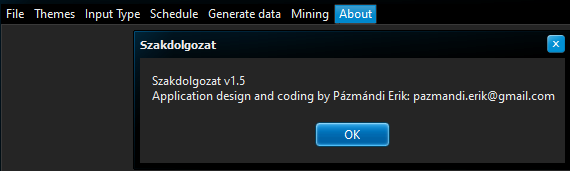
\includegraphics[width=0.5\textwidth, keepaspectratio=true]{images/img_ui_about}\\
				\label{fig:example}
			\end{center}
		\end{figure}
	}

\end{enumerate}

\Section {Folyamathoz tartozó vezérlés}

\Section {Adatbányászat}